\section{Proposed Research}
\label{sec:proposed-work}
This proposal is an outgrowth of the PIs' ongoing successful
collaboration. Building off complementary expertises, the specific aims
of this proposal are: mathematical analysis and three-dimensional
membrane energies (\S\ref{sec:specificaim1}: PI Ryham), BIE
implementation for large granule-number and three-dimensional
suspensions (\S\ref{sec:specificaim2}: PI Quaife), and kinetic theory modeling
(\S\ref{sec:specificaim3}: PI Young).

\subsection{Specific Aim 1: Membrane vesicles as self-organized granules}
\label{sec:specificaim1}
We introduced~\eqref{eq:RBT}--\eqref{eqn:stressbalance} to complement
existing methods for studying vesicles and bilayers. The simulation
results in Figures~\ref{fig:JPv_linearshear} and~\ref{fig:JPv_rupture}
show that two-dimensional, granule-based vesicles replicate the
equilibria and hydrodynamics for continuous curves~\cite{FuQuRyYo22,
Fu2018_SIAM}. Our next goal is to study the model using rigorous
analysis and consider three-dimensional effects. 

The first step is to obtain some solid well-posedness results
for~\eqref{eq:RBT}--\eqref{eqn:stressbalance}. This system is an
autonomous system of ordinary differential equations (ODEs) for the body
transformations $\FF_i$ with the rate of change defined by a system of
PDEs. Strategies have been proposed for the solution of coupled PDE/ODE
systems \cite{Carichino2018EnergybasedOS,Quarteroni2016GeometricMM}.
Regarding \eqref{eq:RBT}--\eqref{eqn:stressbalance}, in the linear case
and for fixed $t$, there is a unique solution ($\phi, \uu$) under
appropriate assumptions for the boundaries and boundary
data~\cite{manasthesis, rac-gre2016, LAX}. These define instantaneous
rigid body velocities and rotations, leading to the following problem.
\begin{quotation}
  \noindent
  \textbf{Problem 1.} 
  Consider a collection of closed, disjoint granules $U_i$ with smooth
  boundary, with no-slip, rigid body motion boundary conditions, and a
  linear background flow. Assume a single-well potential and smooth
  phase field boundary conditions. What is the well-posedness in time of
  the coupled system \eqref{eq:RBT}--\eqref{eqn:stressbalance}?
\end{quotation}
Problem 1 involves mathematically interesting techniques. First, we must
establish that the system has a local-in-time solution. This involves
domain perturbations and estimates for the solutions of second-order
elliptic equations~\cite{Savar2002DomainPA, DANERS20081,
Lamboley2015EstimatesOF}, which also find extensive application in
extremal domain problems~\cite{Schiffer1954VariationOD,
Henrot2006ExtremumPF, bogosel:hal-03607776,Bogosel2022OnTP}, for
example.
For global-in-time solutions, we can use lubrication
forces~\cite{cawthorn_balmforth_2010, leal_2007}. Here, the lubrication
force required to bring granules into contact blows up with distance,
and we must analyze whether the attraction~\eqref{eqn:stressbalance}
stays finite in order to guarantee positivity in the distance between
granules.
Finally, we can study the granule-flow behavior in the
zero-decay length limit. This limit should recover the hydrodynamics of
a (noninteracting) rigid-body suspension.

\begin{wrapfigure}[11]{r}{0.5\textwidth}
  \vspace{-8pt}
  \centerline{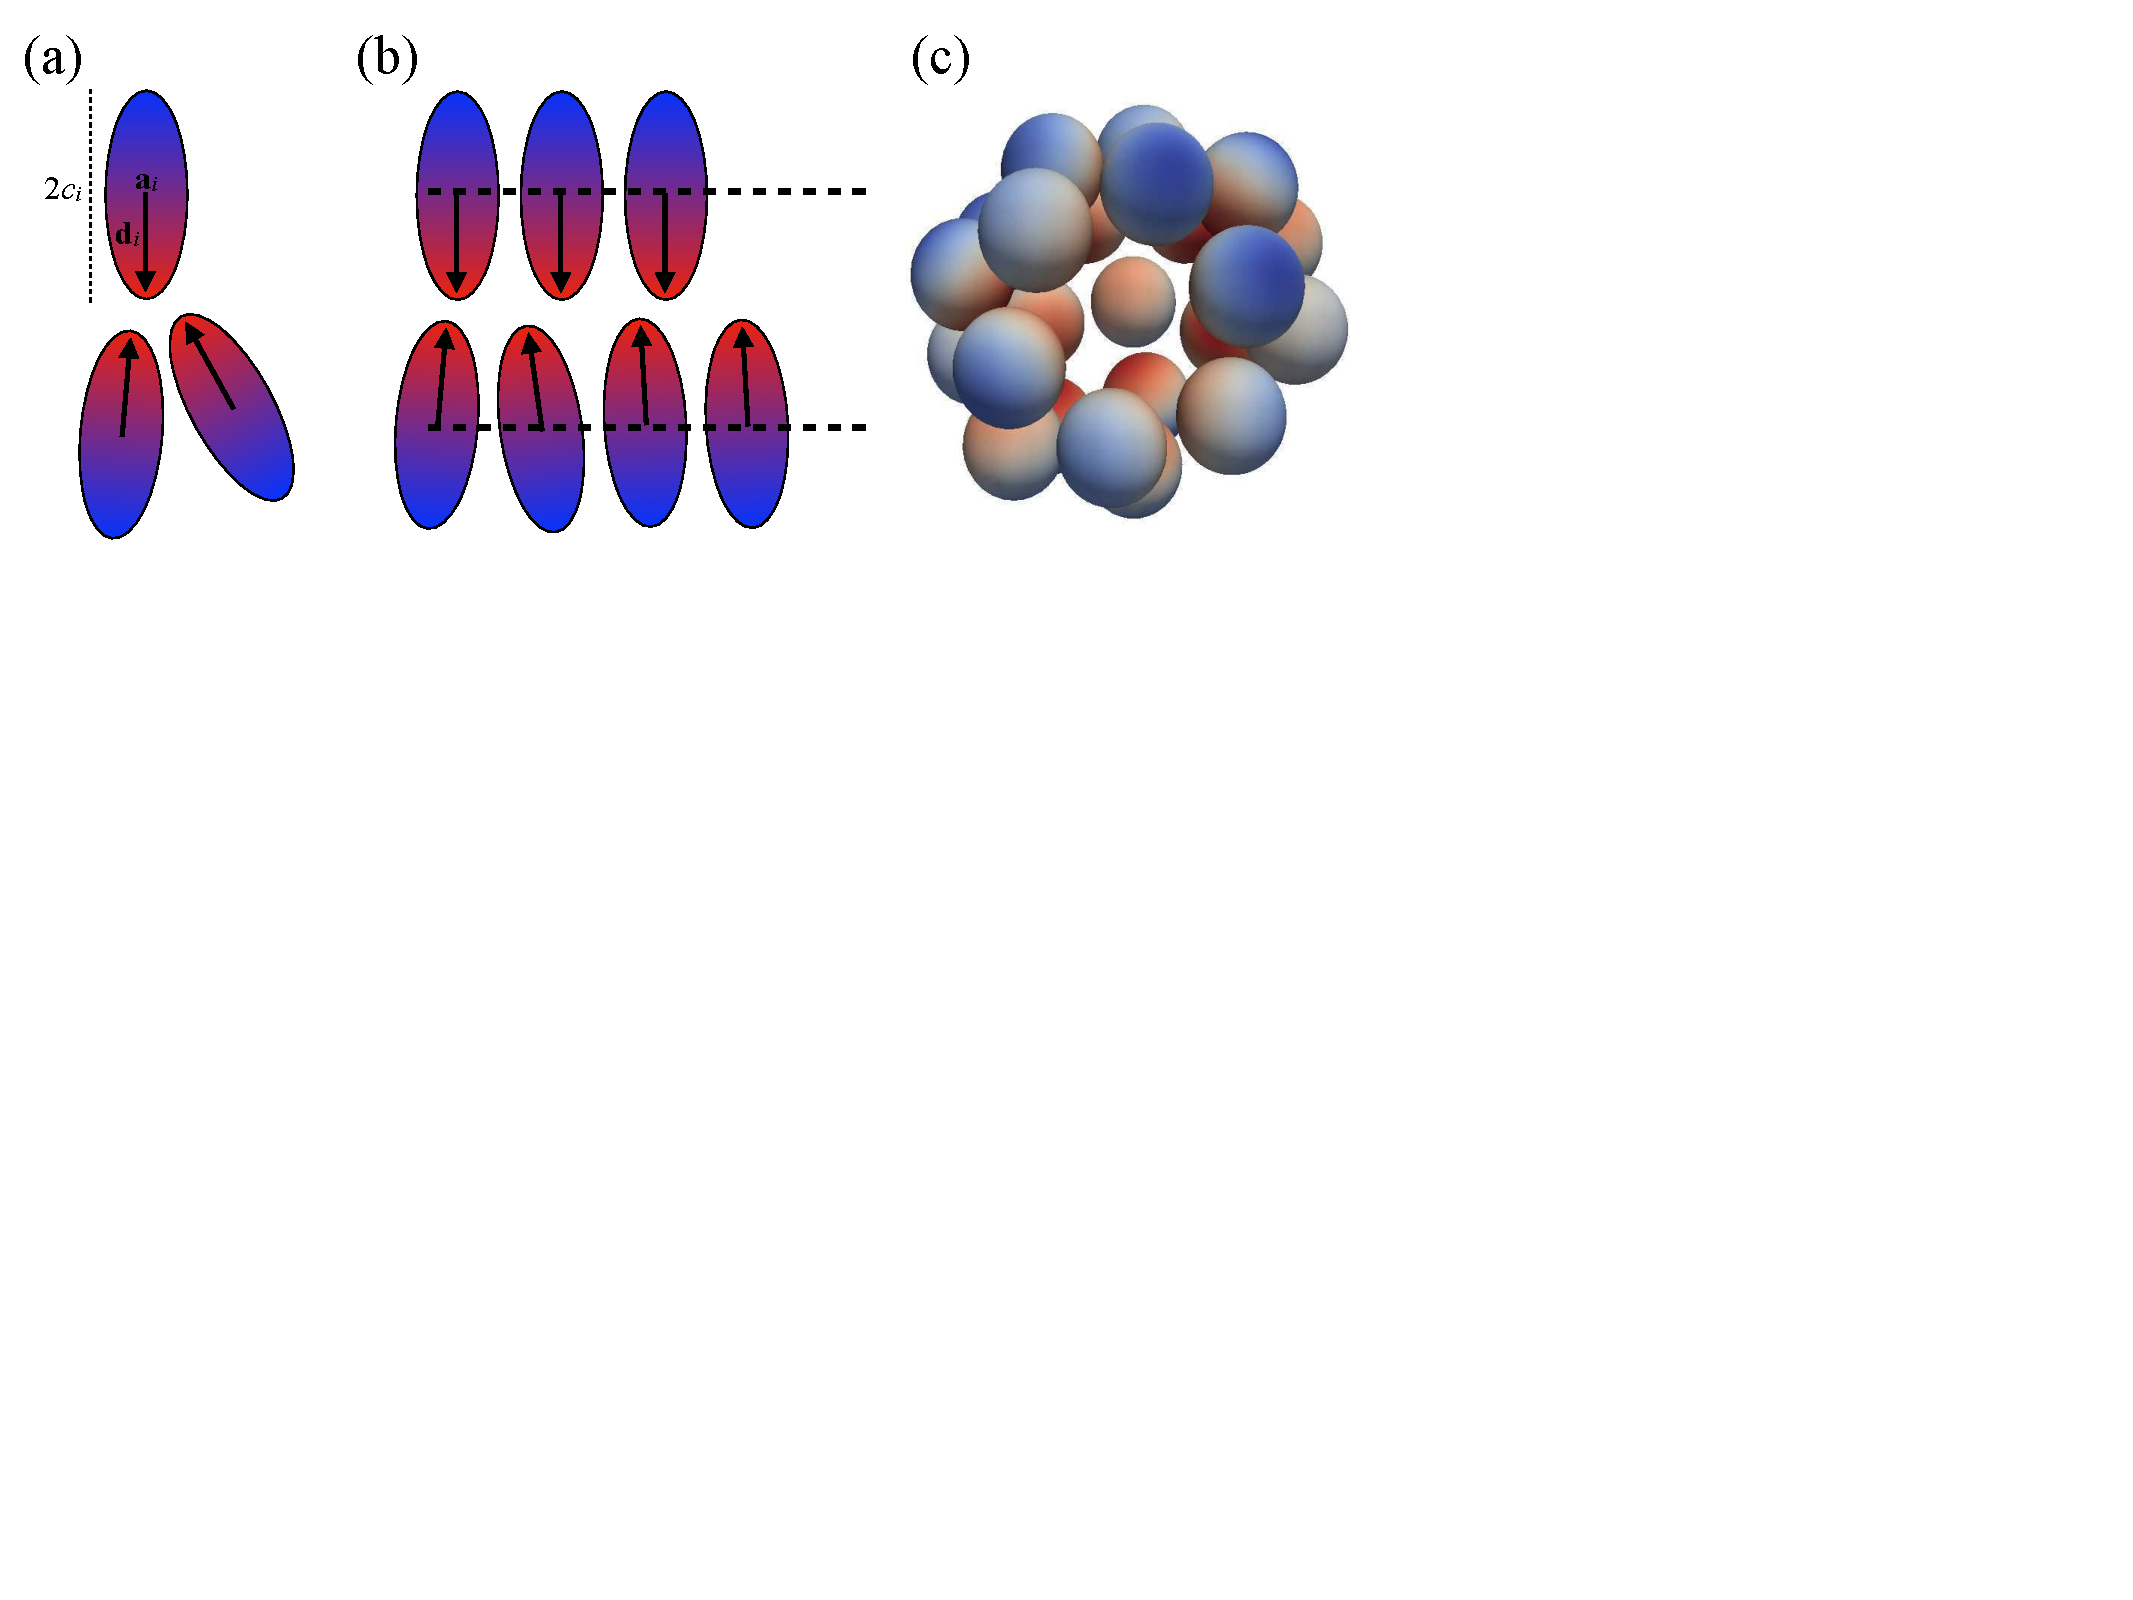
\includegraphics[width=0.5\textwidth]{figures/SA1Figures/AmphiphilicAssembly.pdf}}
  \vspace{-8pt}
  \caption{\label{fig:amphiphilic_assembly} \footnotesize
  Self-organization under an amphiphilic boundary condition. (a)
  Granules first match hydrophobic tails (red), (b) then align
  lengthwise. (c) The same pattern of self-organization holds in three
  dimensions, as simulated by Kohl, Corona, and
  Veerapaneni~\cite{koh-cor-che-vee2021}.}
\end{wrapfigure}
In the double-well potential case, equation~\eqref{eqn:phase} is a
nonlinear Allen-Cahn equation. This situation models granules immersed
in a two-phase fluid (e.g., granules in an emulsion) where there is an
interesting interplay between the long-range alignment of granules and
the diffusive interface energy of the free boundary between fluid
phases. On unbounded domains like $\Omega(t)$, Allen-Cahn equations can
have multiple solutions~\cite{Alama1997StationaryLS,
Alikakos2008OnAE, Bronsard1993OnTB, Byeon2014SolutionsOH, Byeon2013OnAP,
Alessio2005ENTIRESI, Trumper2007ExistenceOA, Benci2019MultipleSF}.
To have one solution $\phi$ for each $t$, 
we must reformulate~\eqref{eqn:phase} as
the following initial value problem with transport:
\begin{align}
  \label{eqn:phase_transport}
  \phi_t + \uu \cdot \nabla
  = -\beta \frac{\delta E}{\delta \phi}
  = \beta(\epsilon^2 \Delta \phi - W'(\phi)),
  \quad \phi(\xx,0) = \phi_0(\xx),
\end{align}
for initial data $\phi_0$. The modified system enjoys an energy law
similar to~\eqref{eq:energy_law} with an additional dissipation term
involving the square the Euler-Lagrange derivative $\frac{\delta
E}{\delta \phi}$ and dampening factor $\beta > 0$. There are several
works dealing with the characterization of the geometric evolution of
interfaces under the Allen-Cahn and Cahn-Hilliard
equations~\cite{Christlieb2019CompetitionAC, Gavish2011CurvatureDF,
Dai2019WeakSF, Promislow2017ExistenceBA, Dai2015CompetitiveGE,
Promislow2012CriticalPO, Dai2022GeometricEO, Dai2020MinimizersFT,
Dai2013GeometricEO, Promislow2022UndulatedBI, Gera2017CahnHilliardOS}
and well-posedness
results when coupled to flow in static domains~\cite{Jiang2017TwophaseIF,
Liu2012StrongSF, Giorgini2019WellPosednessOA, Wu2022WellposednessOA,
Gal2010AsymptoticBO, Giorgini2020DiffuseIM, Giorgini2019UniquenessAR}.
The proposed research extends these results to problems with moving
domains. A closely related and strongly developing direction in the area
of nematic liquid crystals concerns the interaction of Landau-de Gennes
functionals with colloids, and studies the qualitative structure of
defects around single or multiple colloidal
particles~\cite{doi:10.1098/rsta.2020.0432, Alama2015MinimizersOT,
Alama2021SaturnRD, PhysRevE.96.042702}.
PI Ryham has several works on
membrane vesicles dealing both with Allen-Cahn formulations and
fluid-vesicle interactions~\cite{QiangDu09, RYHAM20112929, RyCoEi12,
Ryham2017OnTV}.

The second problem considers the approximation of elastic energy of
curves and surfaces, and seeks to make rigorous the simulation results
of~\cite{FuQuRyYo22, Fu2018_SIAM}. We employ the so-called
``amphiphilic'' boundary condition that leads a collection of
granules to form bilayers. Referring to
Figure~\ref{fig:amphiphilic_assembly}, 
\begin{align}
\label{eq:amphiphilic_BC}
  \phi(\xx) = \tfrac{1}{2}\left(\dd_i \cdot 
    (\xx - \aa_i)/c_i + 1\right), \quad \xx \in \Gamma_i,
\end{align}
where $\dd_i$ is the director, $|\dd_i| = 1$, $\aa_i$ is the center, and
$c_i$ the ``radius'' of the $i$th granule. The phase $\phi$ takes values
close to $1$ in the direction $\dd_i$, representing a hydrophobic tail,
and values close to $0$ in the direction $\dd_i$ representing the
hydrophilic head.

\begin{quotation}
  \noindent
  \textbf{Problem 2.}
  Consider a collection of two-dimensional amphiphilic granules along a
  closed curve $\mathcal{C}$. What is the sharp interface limit of the
  energy $E$ as the number of granules goes to infinity and their size
  to zero?
\end{quotation}
Sharp interface models represent a membrane vesicle as an
inextensible, continuous, closed surface $\Sigma$ with elastic energy
\begin{align}
  \label{eq:Canham-Helfrich}
  \int_{\Sigma} k_B(H - k_0)^2\, dS,
\end{align}
where $H$ is the mean curvature, $k_0$ is a spontaneous curvature, and
$k_B$ is a bending modulus. One can also account
for spatially dependent spontaneous curvature
\cite{PhysRevE.79.031926,Lowengrub13,mahapatra_saintillan_rangamani_2020}
and for extensibility by
including in~\eqref{eq:Canham-Helfrich} an additional stretching term
$k_A(\alpha - \alpha_0)^2/\alpha_0^2$ where $\alpha$ and $\alpha_0$ are
the deformed and equilibrium area densities respectively
\cite{chabanon2017}, and $k_A$ is a stretching modulus.

In the case of granules, bending enters through the splay of the granule
directors. In Figure~\ref{fig:JPv_linearshear}, for example, the
directors have negative, respectively positive, splay $\nabla_{\Sigma}
\cdot \dd$ in the outer, respectively inner monolayers. Here
$\nabla_{\Sigma}\cdot{}$ is the surface divergence. From differential
geometry, we have that $\nabla_{\Sigma} \cdot \dd = \pm 2H$ whenever $\dd$ is
everywhere normal to $\Sigma$, and this is how curvature enters the
granule-based description. For two-dimensional vesicles, $H$ is replaced
with the curvature $\kappa$ of the curve $\mathcal{C}$. Granules are at
rest when attraction balances repulsion, and will have stretching energy
when the distance between neighboring granules is increased from rest.

Tools for addressing Problem 2 have been developed for bulk nematic
liquid crystal potentials in the area of colloidal
homogenization~\cite{Canevari2019DesignOE, doi:10.1137/18M1163919,
BERLYAND200597, doi:10.1137/130910348}, and the problem is closely
related to dimension reduction for curved nematics confined to thin
films~\cite{Golovaty2017DimensionRF, Golovaty2015DimensionRF,
doi:10.1142/S0218202516500470, FoFrLe07}. PI Ryham has carried out sharp
interface-limit analyses for phase field formulations of elastic bending
energy~\cite{0951-7715-18-3-016, Du05}, approximations of Gaussian
curvature and the Euler characteristic in phase field~\cite{DuEuler},
and vanishing Debye-length in Poisson-Boltzman equations~\cite{Lee2018,
1531-3492_2006_2_357}.

Finally, to consider three-dimensional effects, we will generalize
Problem 2 to \emph{numerically} study the energies of amphiphilic
granules confined to surfaces. Recent works on nematics on a surface have
studied the interplay between surface geometry and a director
field~\cite{Nestler2020PropertiesOS, Nitschke2018NematicLC,
Nestler2018OrientationalOO, Nitschke2019HydrodynamicII,
Nitschke2020LiquidCO}. Researchers have formulated finite element
methods~\cite{Bartels2012FiniteEM, Nochetto2015NumericsFL,
Nestler2019AFE} and studied minimizers~\cite{Segatti2014EquilibriumCO,
Segatti2014AnalysisOA}. In biophysics, researchers
have derived the generalized Helfrich energy for lipid bilayers that
involves coupling effects between lipid tilt to director
splay~\cite{Hamm2000ElasticEO, Terzi2019CurvatureTiltTO, Terzi2019ACQ,
  Terzi2017NovelTC, Pinigin2020NewCT,Rangamani20140463}. It contains~\eqref{eq:Canham-Helfrich}
as a special case.
\begin{quotation}
  \noindent
  \textbf{Problem 3.} Simulate surfaces made up of three-dimensional,
  amphiphilic granules. Numerically investigate the limiting energy for
  large-$N_b$ suspensions.
\end{quotation}
We will study Problem 3 by simulating large granule-number membranes.
If, after thoroughly sampling shapes and boundary conditions,
it turns out that the granule energies are not described by
a nematic or Helfrich-type energy, then we will change
hypotheses and look for alternative sharp interface elastic energies.
PI Ryham is well-qualified to lead this investigation.
In his much noticed Biophysical Journal and Nature
papers~\cite{RyKlYaCo16, Chetal16}, he calculated least energy
paths for \emph{membrane fusion} using a surface-director model based on
the general Helfrich energy. The energy barriers 
proved consistent with later results from molecular dynamic
simulation and experiment~\cite{SmRiMu19, 2017PNAS..114.1238F}.

The completion of Problems 1, 2, and especially 3 requires additional
algorithmic implementation including a fast summation method such as the
fast multipole method. The implementation details, in particular how we
deal with large granule numbers and three-dimensional systems are
described in Specific Aim 2 (\S\ref{sec:specificaim2}).




%\begin{equation}
%\label{eq:Helfrich}
%  \begin{aligned}
% &\int_{\Sigma}
%  %\label{eq:Pinigan}
%\tfrac{1}{2}k_{b}[(\nabla_{\Sigma} \cdot \mathbf{d} + k_{0})^{2} -  k^{2}_{0}]  
%+ \tfrac{1}{2}k_{\theta}\mathbf{T}^{2} + \tfrac{1}{2}k_a[(\alpha - \alpha_0)^2 - \alpha_0^2] \\
%&+ k_{c}\textbf{T} \cdot \nabla_{\Sigma} \nabla_{\Sigma} \cdot \mathbf{d}  + \tfrac{1}{2}k_{g}(\nabla_{\Sigma} \nabla_{\Sigma} \cdot \mathbf{d})^{2}
% + A\alpha \nabla_{\Sigma} \cdot \mathbf{d}
%+ B \mathbf{T} \cdot \nabla_{\Sigma} \alpha \\
%&- \tfrac{1}{2}k_c |\nabla_{\Sigma} \alpha|^2 + C \nabla_{\Sigma} \alpha \cdot \nabla_{\Sigma} \nabla_{\Sigma} \cdot \mathbf{d}\,dS
%\end{aligned}
%\end{equation}
%in the lipid director $\dd$,
%tilt vector $\mathbf{T}$
%the difference between the lipid director $\mathbf{d}$ and the surface normal
%$\mathbf{N}$; area per lipid $\alpha$,
%and where $\nabla$ and $\nabla \cdot$ are the surface gradient and surface divergence, respectively. 
%The two models \eqref{eq:Canham-Helfrich} and \eqref{eq:Helfrich} agree
%when $\mathbf{T} = 0$ and $\alpha = \alpha_0$ everywhere.
%The remaining term $k_B$, $k_{\theta}$, $k_a$, $k_c$, $k_g$, $A$, $B$, $C$ are
%appropriate elastic moduli.




